\titledquestion{Multiple Choices}

Each question has \textbf{one or more} correct answer(s). Select all the correct answer(s). For each question, you will get 0 points if you select one or more wrong answers, but you will get 1 point if you select a non-empty subset of the correct answers.

Write your answers in the following table.

%%%%%%%%%%%%%%%%%%%%%%%%%%%%%%%%%%%%%%%%%%%%%%%%%%%%%%%%%%%%%%%%%%%%%%%%%%%
% Note: The `LaTeX' way to answer a multiple-choices question is to replace `\choice'
% with `\choice', as what you did in the previous questions. However, there are 
% still many students who would like to handwrite their homework. To make TA's work 
% easier, you have to fill your selected choices in the table below, no matter whether 
% you use LaTeX or not.
%%%%%%%%%%%%%%%%%%%%%%%%%%%%%%%%%%%%%%%%%%%%%%%%%%%%%%%%%%%%%%%%%%%%%%%%%%%

\begin{table}[htbp]
	\centering
	\begin{tabular}{|p{1.7cm}|p{1.7cm}|p{1.7cm}|p{1.7cm}|p{1.7cm}|p{1.7cm}|p{1.7cm}|p{1.7cm}|p{1.7cm}|}
		\hline
		(a)       & (b)       & (c)      & (d)       & (e)        & (f)      \\
		\hline
		%%%%%%%%%%%%%%%%%%%%%%%%%%%%%%%%%%%%%%%%%%%%%%%%%%%%%%%%%%
		% YOUR ANSWER HERE.
		\hfill BD & \hfill BC & \hfill A & \hfill AC & \hfill ABC & \hfill A \\
		%%%%%%%%%%%%%%%%%%%%%%%%%%%%%%%%%%%%%%%%%%%%%%%%%%%%%%%%%%
		\hline
	\end{tabular}
\end{table}

\begin{parts}
	\part[2] Which of the following is(are) incorrect? ($|V|$ is the number of vertexes, $|E|$ is the number of edges.)
	\begin{choices}
		\choice In DAGs(directed acyclic graphs), A simple path can visit the same vertex twice.
		\correctchoice For a forest, the number of trees is $|V|-|E|$.
		\choice In weighted directed graphs, if both $(v_j, v_k)$ and $(v_k, v_j)$ are edges, it is required that they have the same weight.
		\correctchoice The maximum number of edges in a simple undirected graph is $O(|V|^2)$.
	\end{choices}


	\part[2] If we use the breadth-first algorithm to traverse the following graph, which are the possible orders of visiting the nodes?

	\begin{center}
		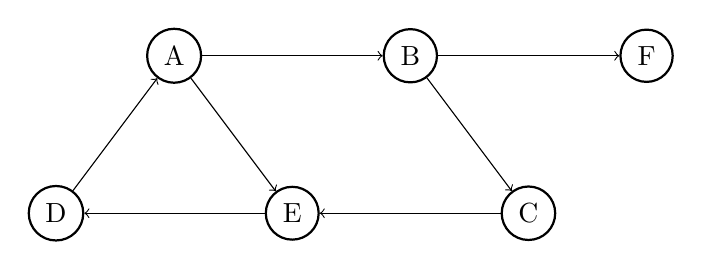
\begin{tikzpicture}
			\begin{scope}[every node/.style={circle,thick,draw}]
				\node (A) at (0,0) {A};
				\node (B) at (3,0) {B};
				\node (F) at (6,0) {F};
				\node (D) at (-1.5, -2) {D};
				\node (E) at (1.5, -2) {E};
				\node (C) at (4.5, -2) {C} ;
			\end{scope}
			\begin{scope}[ every node/.style={fill=white,circle}]
				\path [->] (A) edge (B);
				\path [<-] (A) edge (D);
				\path [->] (A) edge (E);
				\path [->] (E) edge (D);
				\path [->] (B) edge (C);
				\path [->] (B) edge (F);
				\path [->] (C) edge (E);
			\end{scope}
		\end{tikzpicture}
	\end{center}
	\begin{choices}
		\choice BAEDFC
		\correctchoice ABECFD
		\correctchoice DABECF
		\choice ABCEDF
	\end{choices}

	\part[2] Which of the following statements are true for graph traversal? ($|V|$ is the number of vertexes, $|E|$ is the number of edges.)
	\begin{choices}
		\correctchoice Time complexity of DFS and BFS are both \(\Theta(|V| + |E|)\).
		\choice For a directed graph, DFS starting at any vertex can traverse all the nodes.
		\correctchoice Assuming we use a queue to implement BFS. Let \(d(v)\) be the minimum number of edges between \(v\) and \(s\), \(s\) is the start vertex. For any two vertices \(u, v\) in the queue at the same time, \(|d(u) - d(v)| \leq 1\).
		\choice A directed graph with \(n\) nodes and \(2n\) edges is strongly connected.
	\end{choices}

	\part[2] Which of the following statements are true for graph traversal?
	\begin{choices}
		\correctchoice Undirected graph \(G = (V,E)\) is stored in an adjacency matrix A. The degree of \(V_i\) is \(\sum_{j = 1}^{|V|}A[i][j]\). ($A[i][j] = 0, 1$)
		\choice Graph with an odd number of vertices cannot be a bipartite graph.
		\choice If a graph with \(n\) vertices has \(n - 1\) edges, it must be a tree.
		\choice Given two vertices $s$ and $t$ in a graph $G$, we can use both BFS and DFS to determine whether there exists a path from \(s\) to \(t\).
	\end{choices}


	\part[2] Consider a tree with 64 nodes. It is generated by a disjoint set union with union-by-rank (height). Select the possible height(s) of the tree.
	\begin{choices}
		\correctchoice 1
		\correctchoice 2
		\correctchoice 6
		\choice 7
	\end{choices}

	\part[2] Which of the following statements are true for MST(Minimum Spanning Tree)?
	\begin{choices}
		\correctchoice If the weights of the graph are distinct, i.e. every edge has a different weight, the MST of the graph is unique.
		\choice If we use heap or priority queue to optimize Prim's algorithm when choosing the next edge, it will always have a better time complexity than the unoptimized algorithm on any graph.
		\choice Prim's algorithm is a divide-and-conquer algorithm because it divides the graph into $S$ and $V-S$ then solve.
		\choice If we add a new edge$e = (u,v)$ into a graph $G=(V,E)$ with unique MST to get a new graph $G' = (V,E\cup\{e\})$. There is at most $1$ edge difference between the MST of $G$ and $G'$.
	\end{choices}

\end{parts}
